\documentclass[11pt,hyperref={unicode}]{beamer}

\usepackage[slovene]{babel}
\usepackage[utf8]{inputenc}
\usepackage[T1]{fontenc}
\usepackage{lmodern}
\usepackage{graphics}
\usepackage{tikz}

\usetikzlibrary{3d,calc}

\usetheme{Madrid}
% ===================================================================
\title{Priprava prosojnic v LaTeX-u}
\subtitle{Uporaba paketa \texttt{beamer}}
\author{Luka Toplak}
\institute[FMF]{FMF Fakulteta za matematiko in fiziko}
\date{}
% -- -----------------------------------------------------------------
\begin{document}

\frame{\titlepage}

\begin{frame}
   \frametitle{Kratek pregled}
   \tableofcontents[pausesections]
\end{frame}
% ===================================================================
\section{Razporeditev vsebine}
% -------------------------------------------------------------------
\begin{frame}
   \frametitle{Naštevanje}
   
   Za naštevanje lahko uporabimo okolje \texttt{itemize}:
   \begin{itemize} 
      \item Prva točka.
      \item Druga točka.
      \item Tretja točka.
   \end{itemize}
   ali pa okolje \texttt{enumerate}:
   \begin{enumerate}
      \item Prva točka.
      \item Druga točka.
      \item Tretja točka.
   \end{enumerate}
\end{frame}
% -------------------------------------------------------------------
\begin{frame}
   \frametitle{Bloki z naslovom}
   Dele besedila lahko zapišemo v bloke.

   Uporabimo okolja \texttt{block}, \texttt{exampleblock}, \texttt{alertblock}.

   Za parameter okolja napišemo naslov bloka.

   \begin{block}{Opomba}
      Tako je videti block z naslovom.
   \end{block}
   
   \begin{exampleblock}{Primer}
      Tako je videti exampleblock z naslovom.
   \end{exampleblock}

   \begin{alertblock}{Opozorilo}
   Tako je videti alertblock z naslovom.
   \end{alertblock}
\end{frame}
% -------------------------------------------------------------------
\begin{frame}
   \frametitle{Bloki brez naslova}
   Blok lahko ima tudi prazen naslov.
   
   V takem primeru bo brez naslovne vrstice.
   
   \begin{block}{}
      Tako je videti \texttt{block} s praznim naslovom.
   \end{block}
   
   \begin{exampleblock}{}      
      Tako je videti \texttt{exampleblock} s praznim naslovom.
   \end{exampleblock}

   \begin{alertblock}{}
      Tako je videti \texttt{alertblock} s praznim naslovom.
   \end{alertblock}
\end{frame}
% -------------------------------------------------------------------
\begin{frame}
   \frametitle{Stolpci}
   \begin{columns}
      \begin{column}{0.5\textwidth}
         \begin{itemize}
            \item Besedilo lahko pišemo v več stolpcih.
            \item Osnovno okolje je \texttt{columns}.
            \item Posamezen stolpec opišemo v okolju \texttt{column}.
            \item Vsebina stolpca je lahko poljubna.
            \item Za primer imamo v desnem stolpcu napis v bloku in sliko 
            sončnice.
         \end{itemize}
      \end{column}
      \begin{column}{0.45\textwidth}
         \begin{center}
            \begin{exampleblock}{}
               \centering
               Slika v stolpcu.
            \end{exampleblock}
            \includegraphics{soncnica.jpg}
         \end{center}
      \end{column}
   \end{columns}
\end{frame}

% ===================================================================
\section{Matematične trditve}
% -------------------------------------------------------------------
\begin{frame}
   \frametitle{Praštevila}
   \begin{block}{Definicija}
      \textit{Praštevilo je naravno število, ki ima natanko dva delitelja.}
   \end{block}

   \begin{exampleblock}{Zgledi}
      \begin{itemize} 
         \item 1 je praštevilo (ima samo enega delitelja: 1).
         \item 2 je praštevilo (ima dva delitelja: 1 in 2).
         \item 3 je praštevilo (ima dva delitelja: 1 in 3).
         \item 4 ni praštevilo (ima tri delitelje: 1, 2 in 4).
      \end{itemize}
   \end{exampleblock}
\end{frame}   
% -------------------------------------------------------------------
\begin{frame}
   \frametitle{Praštevila}
   \begin{block}{Izrek}
      \textit{Praštevil je neskončno mnogo.}
   \end{block}

   \begin{block}{Dokaz.}
      \begin{itemize} 
         \item Denimo, da je praštevil končno mnogo.
         \item Naj bo p največje praštevilo.
         \item Naj bo q produkt števil 1, 2, $ \dots $, p.
         \item Število $ q+1 $ ni deljivo z nobenim praštevilom, torej je 
         $ q + 1 $ praštevilo.
         \item To je protislovje, saj je $ q + 1 > p $ . $\hfill \square $ 
      \end{itemize}
   \end{block}
\end{frame}   
% ===================================================================
\section{Postopno odkrivanje vsebine}
% -------------------------------------------------------------------
\begin{frame}
   \frametitle{Konstrukcija pravokotnice na premico $ p $ skozi točko $ T $}
   \begin{columns}
      \begin{column}{0.5\textwidth}
         \begin{itemize}
            \item <1->Dani sta premica $ p $  in točka $ T $.
            \item <2->Nariši lok $ k $ s središčem v $ T $.
            \item <3->Premico $ p $ seče v točkah $ A $ in $ B $.
            \item <4->Nariši lok  $ m $ s središčem v $ A $.
            \item <5->Nariši lok $ n $ s središčem v $ B $ in z enakim 
            polmerom.
            \item <6->Loka se sečeta v točki $  C $.
            \item <7->Premica skozi točki $ T $ in $ C $ je pravokotna na 
            $ p $.
         \end{itemize}
      \end{column}
      \begin{column}{0.5\textwidth}
         \begin{center}
            \includegraphics[width=0.8\textwidth,keepaspectratio]{pic1.png}<1>
            \includegraphics[width=0.8\textwidth,keepaspectratio]{pic2.png}<2>
            \includegraphics[width=0.8\textwidth,keepaspectratio]{pic3.png}<3>
            \includegraphics[width=0.8\textwidth,keepaspectratio]{pic4.png}<4>
            \includegraphics[width=0.8\textwidth,keepaspectratio]{pic5.png}<5>
            \includegraphics[width=0.8\textwidth,keepaspectratio]{pic6.png}<6>
            \includegraphics[width=0.8\textwidth,keepaspectratio]{pic7.png}<7>
         \end{center}
      \end{column}
   \end{columns}
\end{frame} 
% -------------------------------------------------------------------
\begin{frame}
   \frametitle{Odkrivanje tabele po vrsticah}
   \begin{columns}
      \begin{column}{0.5\textwidth}
         \begin{tabular}{c|cccc}
            Oznaka & A & B & C & D  \\ 
            \hline \onslide<1->
            \onslide<2-> X & 1 & 2 & 3 & 4  \\
            \onslide<3-> Y & 3 & 4 & 5 & 6  \\
            \onslide<4-> Z & 5 & 6 & 7 & 8 
         \end{tabular}
      \end{column}
      \begin{column}{0.5\textwidth}
      \end{column}
   \end{columns}
\end{frame}
% -------------------------------------------------------------------
\begin{frame}
   \frametitle{Odkrivanje tabele po stolpcih}
   \begin{columns}
      \begin{column}{0.5\textwidth}
         \begin{tabular}{c|cccc}
            \onslide<1-> Oznaka & \onslide<2-> A & \onslide<3-> B & \onslide<4-> C & \onslide<5-> D \onslide<1-> \\
            \hline \onslide<1->
            \onslide<1-> X & \onslide<2-> 1 & \onslide<3->2 & \onslide<4-> 3 & \onslide<5-> 4  \\
            \onslide<1-> Y & \onslide<2-> 3 & \onslide<3-> 4 & \onslide<4-> 5 & \onslide<5-> 6  \\
            \onslide<1-> Z & \onslide<2-> 5 & \onslide<3-> 6 & \onslide<4-> 7 & \onslide<5-> 8 
         \end{tabular}
      \end{column}
      \begin{column}{0.5\textwidth}
      \end{column}
   \end{columns}
\end{frame}
% ===================================================================
\section{Razno}
\begin{frame}
   \begin{columns}
      \begin{column}{\textwidth}
         \begin{center}
            \only<1>{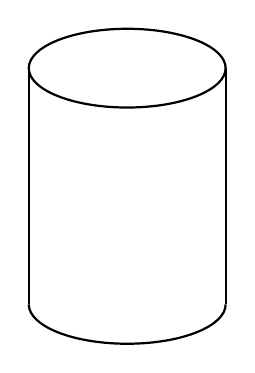
\begin{tikzpicture}<1>
               \draw[thick] (0,0) ellipse (1.25 and 0.5);
               \draw[thick] (-1.25,0) -- (-1.25,-3.0);
               \draw[thick] (-1.25,-3.0) arc (180:360:1.25 and 0.5);
               \draw[thick] (1.25,-3.0) -- (1.25,0);  
            \end{tikzpicture}}
            \only<2>{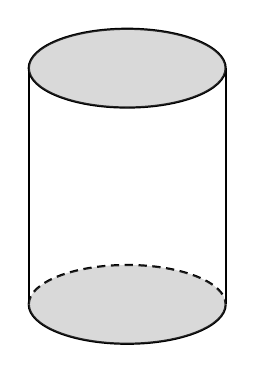
\begin{tikzpicture}<2>
               \draw[thick] (0,0) ellipse (1.25 and 0.5);
               \draw[thick] (-1.25,0) -- (-1.25,-3.0);
               \draw[thick] (-1.25,-3.0) arc (180:360:1.25 and 0.5);
               \draw[thick][densely dashed] (-1.25,-3.0) arc (180:360:1.25 and -0.5);
               \draw[thick] (1.25,-3.0) -- (1.25,0);  
               \fill [gray,opacity=0.3] (1.25,0) arc (0:360:1.25 and -0.5) -- (1.25,-3.0) arc (0:360:1.25 and -0.5);
            \end{tikzpicture}}
            \only<3>{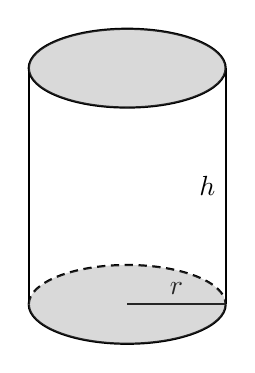
\begin{tikzpicture}
               \draw[thick] (0,0) ellipse (1.25 and 0.5);
               \draw[thick] (-1.25,0) -- (-1.25,-3.0);
               \draw[thick] (-1.25,-3.0) arc (180:360:1.25 and 0.5);
               \draw[thick][densely dashed] (-1.25,-3.0) arc (180:360:1.25 and -0.5);
               \draw[thick] (1.25,-3.0) to [edge label = $ h $] (1.25,0);
               \draw[thick] (0,-3.0) to [edge label = $ r $] (1.25,-3.0);   
               \fill [gray,opacity=0.3] (1.25,0) arc (0:360:1.25 and -0.5) -- (1.25,-3.0) arc (0:360:1.25 and -0.5);
            \end{tikzpicture}}
         \end{center}
      \end{column}
   \end{columns}
\end{frame}
% -------------------------------------------------------------------
\end{document}

% ===================================================================

